% !TeX root = ../main.tex
\chapter{仿真实验}
仿真实验分为三步,首先在Matlab中基于s-function和simulink仿真,验证控制算法的性能;然后在ros框架下,基于PX4固件,修改其运动控制部分的代码,在gazebo中进行软件在环仿真(SITL,software in the loop);接着,将修改后的PX4固件烧写到pixhawk飞控板中,进行硬件在环仿真(HITL,hardware in the loop),而这个版本的固件也可以直接用于后续的实机实验。
\section{Matlab仿真}
我们在Simulink环境下构建了一个综合仿真模型,该模型不仅包含了刚体动力学和电机动态,还通过s-function实现了姿态环和位置环分离的双环控制器设计。这种设计使得后续的数据分析和研究工作能够更为便捷、高效。

为了能直观地体现性能,我们设计了一个“8”字型轨迹,如图\ref{fig:8}:
$$x_d = \begin{matrix}[3\sin(\frac{t}{2}), & 3\cos(\frac{t}{2})\sin(\frac{t}{3}), &-0.1t]\end{matrix}
\quad
\psi_d=0.01t$$

\begin{figure}[!h]
  \centering
  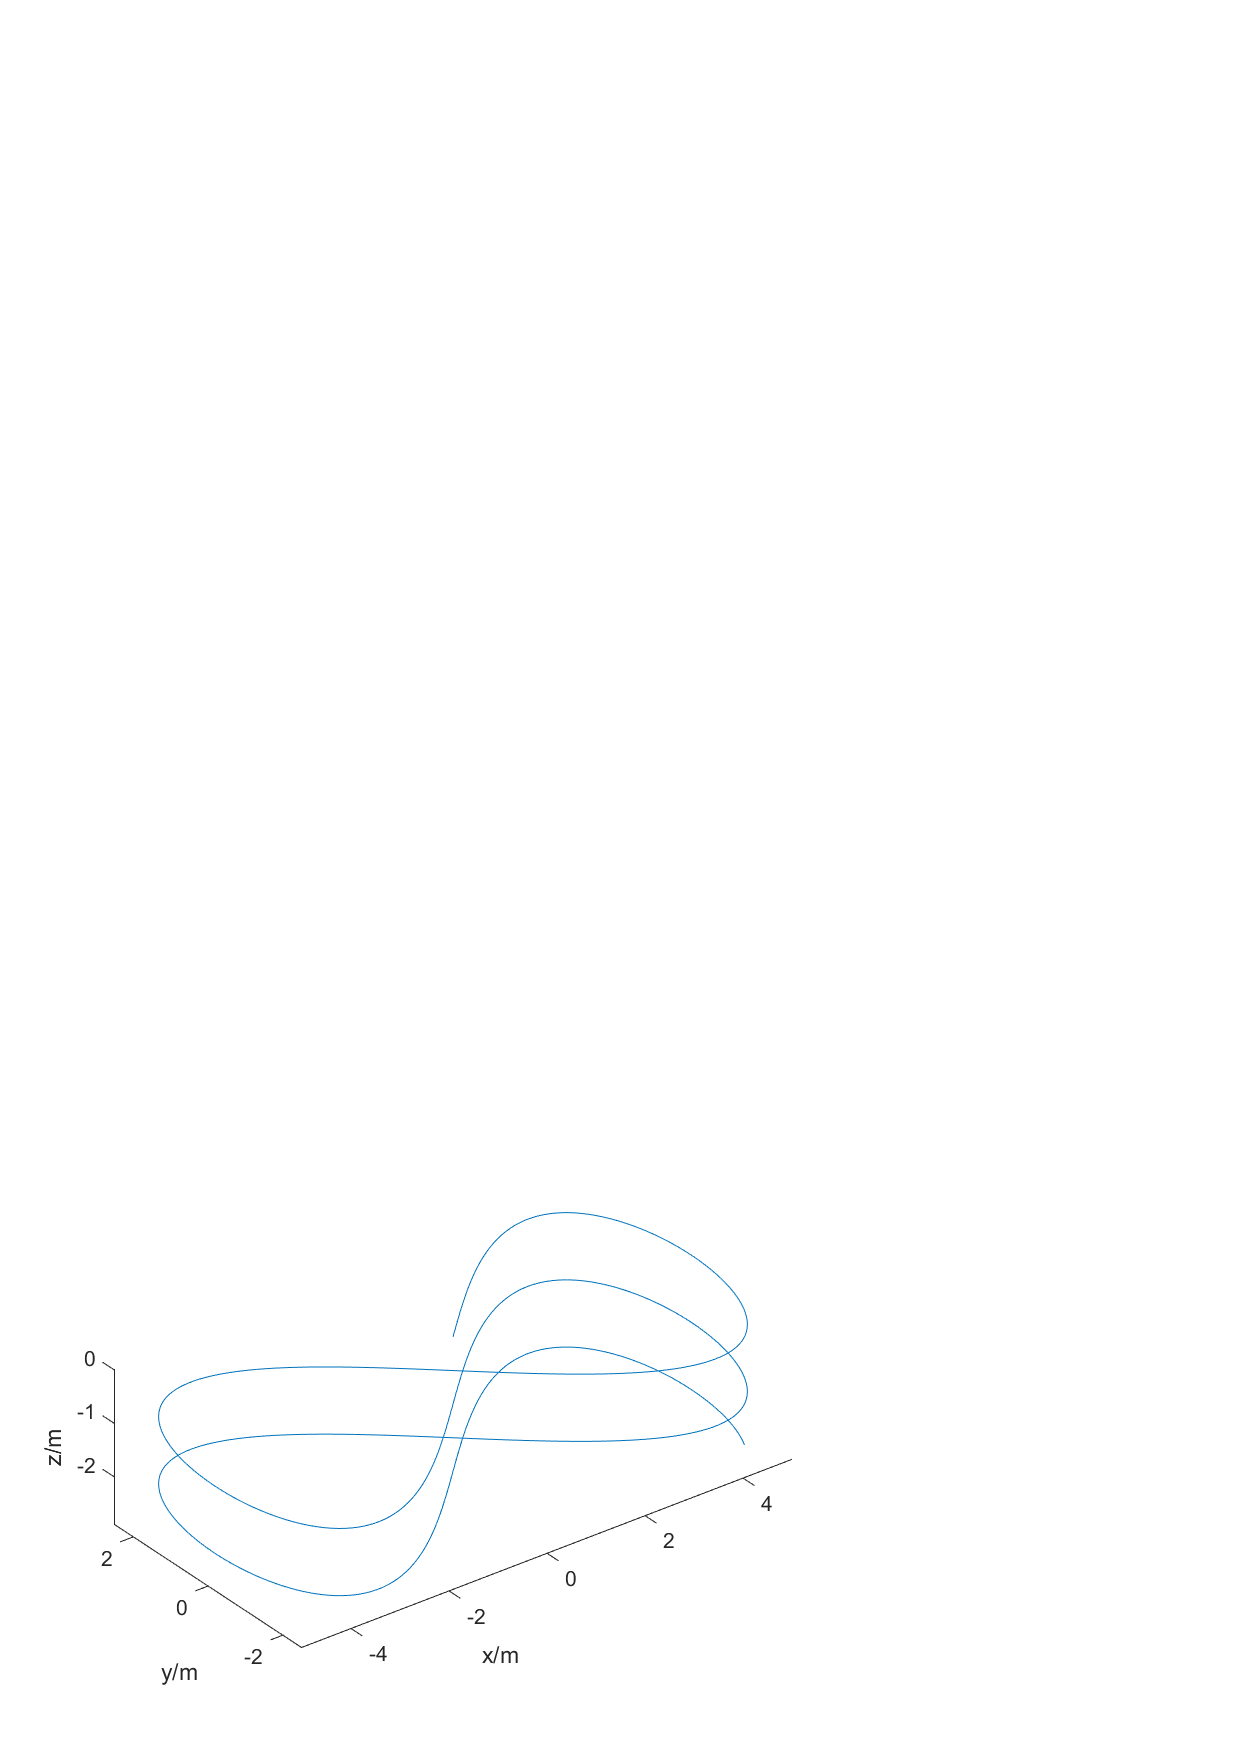
\includegraphics[width=0.5\textwidth]{88.png}
  \caption{高度匀速上升的“8”字型轨迹(北-东-地坐标系下,地面以上Z轴为负数)}
  \label{fig:8}
\end{figure}

为了全面体现控制算法的跟踪性能,我们并没有对轨迹做特殊的平滑处理,轨迹的导数存在间断点使得高阶导数无穷大,这可以考验无人机在现实中的抗扰性能。为了模拟起飞和悬停,第一秒内轨迹保持在原点不动,否则仿真就会等同在空中释放电机无转速的无人机。


  无人机的刚体动力学部分由simulink中自带的“6DOF block”解决,避免了$SO(3)$群差分近似后单位化的困难。该模块会对外部输入的力和力矩做出反应,返回所需的速度、位置、姿态、角速度等信息。

  电机部分,转速的动态由一阶惯性环节表示,根据所选电机型号时间常数$\tau=0.01s$。
  姿态控制器和位置控制器分开由两个s-function实现,重力由单独的模块输入到“6DOF block”。
  \begin{figure}[!h]
    \centering
    \includegraphics[width=0.9\textwidth]{sim.png}
    \caption{simulink仿真连线图}
    \label{fig:sim}
  \end{figure}

  四旋翼无人机的参数由测量和理论计算共同得到:
  $$m=0.8kg \quad d=0.125m \quad J=\begin{bmatrix}
    0.0024   &      0  &       0\\
    0 &   0.0025      &   0\\
    0  &       0   & 0.0041
  \end{bmatrix}kg m^2$$

  电机参数由厂家数据得到:
  $$k_t=2.03\times 10^{-8} \quad 
  \tau=0.01s \quad
  c_{\tau f}=8\times 10^{-3}$$

  选择替补姿态控制律:
  $$k_R=0.881 \quad k_\omega=0.254$$

  由于位置环和姿态环补偿后得到的线性系统A矩阵完全一致,因此选择相同的LQR权重矩阵:
  $$Q=\begin{bmatrix}
    3&0&0&0&0&0\\
    0&3&0&0&0&0\\
    0&0&3&0&0&0\\
    0&0&0&1&0&0\\
    0&0&0&0&1&0\\
    0&0&0&0&0&1\\
  \end{bmatrix} \quad R=\begin{bmatrix}
    0.1 &0 &0\\
    0 &0.1 &0\\
    0 &0 &0.1\\
  \end{bmatrix}$$

  初始位姿:
  $$x(0)=[0,0,0],\quad v(0)=[0,0,0]$$
  $$R(0)=I , \quad \omega(0)=[0,0,0]$$

  按照上述参数,在matlab中用0.005s的控制周期运行仿真,得到结果如图\ref{fig:result-x},\ref{fig:result-angle},\ref{fig:result-f}:
  \begin{figure}[h]
    \centering
    \begin{minipage}[c]{0.33\textwidth}
      \centering
      \includegraphics[width=0.95\linewidth]{result-x.png}
      \caption{位置跟踪效果}
      \label{fig:result-x}
    \end{minipage} \hfill
    \begin{minipage}[c]{0.33\textwidth}
      \centering
      \includegraphics[width=0.95\linewidth]{result-angle.png}
      \caption{角度跟踪效果}
      \label{fig:result-angle}
    \end{minipage}\hfill
      \begin{minipage}[c]{0.33\textwidth}
        \centering
        \includegraphics[width=0.95\linewidth]{result-f.png}
        \caption{四个电机输出的力}
        \label{fig:result-f}
    \end{minipage}
    \end{figure}

  从以上图中可以看到本控制算法可以很好地跟踪这种有较大姿态机动的轨迹,只是由于轨迹在起始时存在阶跃,导致无人机在阶跃处需要一定的动态过程才能跟踪上。但是在实际的飞行任务中,在轨迹规划层面就需要对轨迹做光滑处理。为了避免出现执行器饱和的情况,在仿真中我们根据无人机的实际情况和电机所能输出的最大升力,设置了控制器输出力和力矩的上限。

  \pagebreak
  
  三维空间下的轨迹跟踪情况如图\ref{fig:result-3d}

  可以看到在起始的阶跃之后,跟踪效果都十分完美,为了量化地展示跟踪效果,我们提出了平均距离误差和平均偏航角误差:
  $$e_d=\frac{\sum_0^{T}||x-x_d||}{T} \quad e_\psi=e_d=\frac{\sum_0^{T}|\psi-\psi_d|}{T}$$

  误差曲线如图\ref{fig:result-e}
 

  \begin{figure}[h]
    \centering
       \begin{minipage}[c]{0.45\textwidth}
        \centering
        \includegraphics[width=0.9\textwidth]{result-3d.png}
        \caption{三维空间下的轨迹跟踪情况}
        \label{fig:result-3d}
     \end{minipage}%
       \begin{minipage}[c]{0.45\textwidth}
        \centering
        \includegraphics[width=0.9\textwidth]{result-e.png}
        \caption{平均距离误差和平均偏航角误差}
        \label{fig:result-e}
     \end{minipage}
   \end{figure}

   为了体现本控制方法的优越性,设置对照组,与\cite{Lee2010}中也就是上文所说的替补姿态控制律对比(位置环相同):
   
  \begin{figure}[h]
    \centering
    \begin{minipage}[c]{0.33\textwidth}
      \centering
      \includegraphics[width=0.95\linewidth]{com-x.png}
      \caption{对照组位置跟踪效果}
      \label{fig:com-x}
    \end{minipage} \hfill
    \begin{minipage}[c]{0.33\textwidth}
      \centering
      \includegraphics[width=0.95\linewidth]{com-angle.png}
      \caption{对照组角度跟踪效果}
      \label{fig:com-angle}
    \end{minipage}\hfill
      \begin{minipage}[c]{0.33\textwidth}
        \centering
        \includegraphics[width=0.95\linewidth]{com-f.png}
        \caption{对照组四个电机输出的力}
        \label{fig:com-f}
    \end{minipage}
    \end{figure}

    \begin{figure}[h]
      \centering
         \begin{minipage}[c]{0.45\textwidth}
          \centering
          \includegraphics[width=0.9\textwidth]{com-3d.png}
          \caption{对照组三维空间下的轨迹跟踪情况}
          \label{fig:com-3d}
       \end{minipage}%
         \begin{minipage}[c]{0.45\textwidth}
          \centering
          \includegraphics[width=0.9\textwidth]{com-e.png}
          \caption{对照组平均距离误差和平均偏航角误差}
          \label{fig:com-e}
       \end{minipage}
     \end{figure}

     从图\ref{fig:com-3d}中可以直观地看到其跟踪始终有误差未能弥合,在阶跃处同样需要一个动态过程。图\ref{fig:com-f}显示,其推力始终有剧烈抖动,这有可能是因为姿态环的参数调节欠缺。但这正体现了HOFA方法的优越性,相比于对照组的参数调节缺乏理论指导,只能根据经验多次尝试,HOFA方法能将非线性部分全部补偿掉,留下的线性系统对LQR参数并不敏感,权重矩阵并不需要精细地多次调解就能取得很好的控制效果。
     \begin{table}
      \centering
      \begin{tabular}{ccc}
          \toprule
          & 平均距离误差 & 平均偏航角误差 \\
          \midrule
          HOFA方法 & 0.0692 & 0.0072 \\
          对照组 & 0.1580 & 0.0065 \\
          \bottomrule
      \end{tabular}
      \caption{HOFA方法与对照组的平均误差对比}
  \end{table}

  量化的误差指标同样显示,在位置跟踪上,HOFA大幅领先于对照组。在偏航角误差的指标上,有小幅落后,但两者的误差都已经很小。

\section{软件在环仿真}
Matlab仿真只是初步验证了HOFA方法的有效性,既没有考虑实际的飞控固件中异步的采样周期、进程管理等因素,也没有考虑内部和外部传感器信息融合的因素。而在ros+gazebo下的软件在环仿真会考虑以上因素,进一步贴近实际情况。

\subsection{环境配置}
由于当前ros2适配的各种依赖库包括PX4的版本都还在不停迭代,因此目前还是选择更为稳定、资料更多的ros1。在ubuntu20.04中安装ros1 noetic以及配套的mavros和gazebo11 classic,然后从GitHub上clone最近的发行版PX4 v1.14.0,注意要使用递归将所有子项目克隆下来。
\begin{lstlisting}[language=Bash, basicstyle=\footnotesize, linewidth=\linewidth]
  git clone -b v1.14.0 https://github.com/PX4/PX4-Autopilot.git --recursive
\end{lstlisting}

然后运行以下命令以解决依赖。

\begin{lstlisting}[language=Bash, basicstyle=\footnotesize, linewidth=\linewidth]
  Bash Tools/setup/ubuntu.sh
\end{lstlisting}

最后运行软件在环仿真命令:

\begin{lstlisting}[language=Bash, basicstyle=\footnotesize, linewidth=\linewidth]
  make px4_sitl gazebo-classic
\end{lstlisting}

运行成功后会进入gazebo仿真界面,打开QGC会自动连接地面站,在地面站中可以方便地看到回传的位姿信息并且发布起飞和指点飞行命令,如图 \ref{sitl}。在使用gazebo仿真时,需要安装显卡驱动,否则画面渲染将完全使用CPU,这会导致严重的卡顿。

\begin{figure}[h]
  \centering
     \begin{minipage}[c]{0.45\textwidth}
      \centering
      \includegraphics[width=0.9\textwidth]{sitl1.png}
   \end{minipage}%
     \begin{minipage}[c]{0.45\textwidth}
      \centering
      \includegraphics[width=0.9\textwidth]{sitl2.png}
   \end{minipage}
   \caption{SITL gazebo界面以及QGC指点控制}
   \label{sitl}
 \end{figure}

 这里默认使用的是内置的iris无人机模型,有关该模型的具体参数可以在源码\cite{iris}中查到:
 \begin{lstlisting}[language=Bash, basicstyle=\footnotesize, linewidth=\linewidth]
  <inertial>
    <pose>0 0 0 0 0 0</pose>
    <mass>1.5</mass>
    <inertia>
      <ixx>0.029125</ixx>
      <ixy>0</ixy>
      <ixz>0</ixz>
      <iyy>0.029125</iyy>
      <iyz>0</iyz>
      <izz>0.055225</izz>
    </inertia>
  </inertial>

...

<box>
  <size>0.47 0.47 0.11</size>
</box>
 \end{lstlisting}
 
 但因为gazebo下的软件以及硬件在环仿真都只是为了验证算法并且生成在实机上使用的固件,因此不会关注iris模型本身。由于HOFA方法对模型参数的精确性要求不高,且iris和本课题中搭建的四旋翼尺寸重量也大致相当,下一小节中代码里会使用实机重量和转动惯量作为参数。

 \subsection{HOFA算法植入}
在环境配置完成后,接下来就要在PX4源码的基础上修改多旋翼运动控制部分的代码,将其原本的“位置-速度-角度-角速度”四环PID控制 \cite{px4控制}改为HOFA控制。PX4是一个适用于固定翼、直升机、四旋翼、地面车辆乃至于船舶等多种形式机器人的自动驾驶仪,既可以进行软件仿真,也能将固件烧写到硬件中进行实机实验,其架构十分复杂。在多旋翼部分中,就包含多渠道的传感器信息订阅和融合、多个节点间信息的传递,支持实时在地面站修改各种控制参数,支持包含自稳、高度、位置和offboard等多种飞行模式。因此PX4拥有庞大的规模和错综复杂的上层架构,因此在算法植入时,我们将尽可能不改动上层架构,在相应的包内尽量保持输入输出接口不变,避免引起未知的错误。

\textbf{位置环}

PX4的多旋翼位置环控制位于src/modules/mc\_pos\_control包中,包内层次结构如图\ref{mc_pos}。MulticopterPositionControl.cpp和MulticopterPositionControl.hpp主要负责与外部的消息传递,用其Run()函数启动一个位置环(包括位置和速度)控制的进程,其真正的控制代码在mc\_pos\_control/PositionControl/PositionControl.cpp以及其对应的头文件中。

\begin{figure}[!h]
  \centering
  \includegraphics[width=0.3\textwidth]{mc_pos.png}
  \caption{mc\_pos\_control包结构}
  \label{mc_pos}
\end{figure}

位置环的植入较为容易,不需要新定义任何变量,即可在原来的架构上修改。无人机质量直接在代码中写入,因为原本PX4的控制方法并不需要质量信息,因此没有预留可供地面站中可以实时修改的质量参数。而位置和速度的控制律,也就是LQR结算得到的K(只在对角线有非零值),因此可以借MPC\_XY\_P、MPC\_Z\_P、MPC\_XY\_VEL\_P\_ACC、MPC\_Z\_VEL\_P\_ACC这四个参数作为变量载体。由于实机的前后和左右也基本对称,xy轴可以使用同样的参数。这么做的好处在于可以在地面站对这些参数进行实时的调整。

位置环的输出除了期望的推力矢量,还有根据期望推力矢量和期望偏航角生成的期望姿态,这部分函数在ControlMath.cpp中。PX4这部分算法的逻辑与HOFA中的完全一致,也就不需要更改。

\textbf{姿态环}

PX4的多旋翼姿态环控制分别在mc\_att\_control和mc\_rate\_control两个包内,两者间通信的管道是mc\_att\_control向mc\_rate\_control发布期望的角速度“rate\_setpoint”,为了尽量不更改架构,我们接下来也将沿用这一通信管道。

原本的控制算法不需要前一时刻的期望姿态,因此首先要在AttitudeControl.hpp中定义新的变量,包括前一时刻的期望姿态,以及期望姿态订阅时的时间,使用全局配置的drv\_hrt.h中的hrt\_absolute\_time()获得当前函数执行时的时刻。

然后在AttitudeControl.cpp中植入HOFA的核心部分。四元数和旋转矩阵的运算函数在namespace matrix下都有定义,不用自己定义。最终将计算得出的除了$\omega \times J\omega$的期望力矩通过“rate\_setpoint”的传输通道,传递给mc\_rate\_control。无人机的转动惯量参数和姿态控制律的具体数字,直接在AttitudeControl.cpp中定义。如果后续需要调试,则要在源码上进行修改。

进一步在mc\_rate\_control阅读代码,发现包内的MulticopterRateControl.cpp主要做了线程管理和消息更新的工作,真正的控制算法在其Run()函数中调用的RateControl::update()中,这个类函数位于src/lib/rate\_control/rate\_control.cpp。然后就在这个函数中略加修改,完成整个HOFA算法的植入。

\textbf{总结}

总共在四个代码文件中做了修改,分别是:
\begin{itemize}
  \item src/modules/mc\_pos\_control/PositionControl/PositionControl.cpp
  \item src/modules/mc\_att\_control/AttitudeControl/AttitudeControl.hpp
  \item src/modules/mc\_att\_control/AttitudeControl/AttitudeControl.cpp
  \item src/lib/rate\_control/rate\_control.cpp
\end{itemize}

用修改过的这四个文件替换先前环境配置环节中编译完成的包中对应的文件(由于用于修改的代码文件下载时没有递归下载子项目,无法直接编译,且在原本已经过编译的文件夹上修改会更稳妥),再运行make px4\_sitl gazebo-classic命令即可,效果与图\ref{sitl} 基本相同。两种控制方法的定量对比会在实机实验时展开,此处只是粗略验证可行性。

\subsection{硬件在环仿真}
硬件在环仿真的主要目的在于,在gazebo仿真环境中初步测试生成的固件代码,防止直接进行实机实验可能出现的破坏性故障。硬件在环仿真也要首先配置环境,用PX4的发行版跑通流程;然后向飞控刷入植入HOFA的固件,进行硬件在环仿真。

\textbf{环境配置}

硬件在环仿真在软件在环仿真已经跑通的基础上并不困难,PX4的官方文档也提供了相对全面的流程\cite{px4hitl}。

首先用USB连上飞控,在QGC中进行设置:使能HITL;机架选择HITL兼容的Generic Quadcopter,重启;在应用设置中的自动连接选项,仅选择UDP,这一步做完后,直接用USB连接飞控将无法自动连入地面站。以上步骤做完后,断开飞控连接并关闭地面站。

然后是在PX4\_Autopilot包内做软件上的配置,具体代码如下\cite{px4hitl}。

\begin{lstlisting}[language=Bash, basicstyle=\footnotesize, linewidth=\linewidth, breaklines=true]
  cd PX4_Autopilot
  source Tools/simulation/gazebo-classic/setup_gazebo.bash $(pwd) $(pwd)/build/px4_sitl_default
  gazebo Tools/simulation/gazebo-classic/sitl_gazebo-classic/worlds/hitl_iris.world
\end{lstlisting}


需要注意的是,在最后一步run gazebo时,飞控需要已经通过USB连在电脑上。然后打开QGC,即可进行起飞和指点飞行,如图\ref{hitl}所示。
\begin{figure}[!h]
  \centering
  \includegraphics[width=0.6\textwidth]{hitl.jpg}
  \caption{硬件在环仿真示意图}
  \label{hitl}
\end{figure}